
\section{Implementierungsdetails der Operationen} \label{sec:impldetails}
\subsection{Addition und Subtraktion}
    Da Subtraktion bezüglich Addition implementiert ist, werden beide Operationen hier gemeinsam behandelt.

    \paragraph*{Wichtige Funktionen}
        \begin{itemize} \tightlist
            \item \ilc{MPint::carry\_ripple\_add\_bins\_inplace(\&mut self, \dots) -> bool}
            \item \ilc{MPint::overflowing\_add(\&mut self, \dots) -> bool}
            \item \ilc{MPint::twos\_complement\_inplace(\&mut self)}
        \end{itemize}

    \paragraph*{Carry-Ripple-Adder}
        Prinzipiell funktioniert die implementierte Addition wie eine Reihenschaltung von ,,\ilc{u64}-Volladdierern'' (vgl. \autoref{fig:fulladderchain}).

        Die Ziffern $a_i$ und $b_i$ der Summanden $a=a_{n}a_{n-1}\dots{}a_{1}a_{0}$ und $b=b_{n}b_{n-1}\dots{}b_{1}b_{0}$ werden dabei jeweils mit Übertrag\footnote{i.A. kann bei einer Addition höchstens ein Übertrag entstehen, der genau eine Ziffer benötigt ($\hat{=}$ 1 Bit)} addiert.
        $c_i$ wird bei Addition des nächsten Ziffernpaares wieder in den Volladdierer eingespeist usw.

        Die Summe $s=a+b$ ist also:
        \begin{align*}
        s = s_{n+1}s_{n}\dots{}s_{1}s_{0} \quad
            \text{mit:} \quad
                s_i &= (a_i + b_i + c_{i-1}) \mod B \\
                c_i &= \lfloor (a_i + b_i) \div B \rfloor \\
                  B &= 2^{64}
        \end{align*}

        \begin{figure}[H]
            \centering
            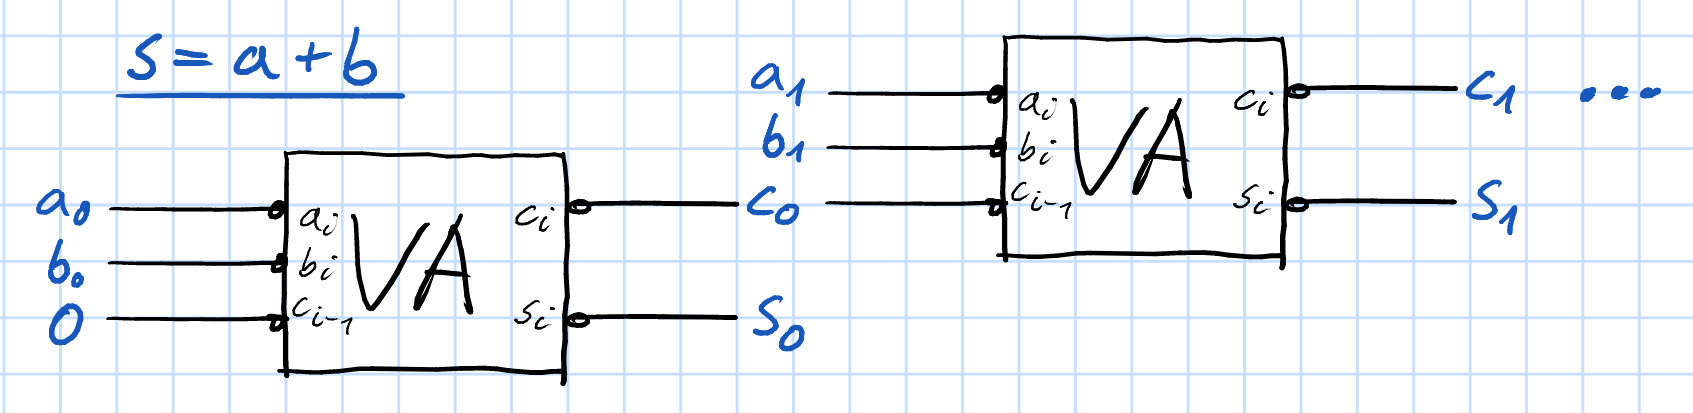
\includegraphics[width=0.7\linewidth]{images/fulladderchain}
            \caption{Addition von \mpi\ mittels Volladdierern}
            \label{fig:fulladderchain}
        \end{figure}

        Abstrakt betrachtet entspricht dieses Konzept einem sog. \emph{Carry-Ripple-Addierer}.

    \paragraph*{Gleiche Vorzeichen}
        Da Vorzeichen und absoluter Wert intern unabhängig voneinander gespeichert sind, kann die Summe bei gleichen Vorzeichen ohne Weiteres, wie oben beschrieben, berechnet werden.

    \paragraph*{Unterschiedliche Vorzeichen}
        Unterscheiden sich die Vorzeichen, sind weitere Schritte erforderlich. Hier tritt eine tatsächliche Subtraktion auf.


        Dank der binären Repräsentation und Eigenschaften des 2-Komplements ist es möglich die Subtraktion auf eine Addition zurückzuführen.
        Hierzu kann man zur Vereinfachung die Summanden erst einmal so ,,ordnen'', dass $a$ immer  der positive und $b$ der negative Summand ist ($a \ge 0$, $b \le 0$). Man kann die Operation dann aufschreiben als:
        \begin{equation*}
        s = a - |b|
        \end{equation*}

        Sei nun $b^*$ das 2-Komplement von $b$, dann berechnet sich $s$ zu:

        \begin{itemize} \tightlist
            \item Falls $a \ge |b|$: (\emph{$s$ positiv})
                \begin{align*}
                    & s = a + b^*
                \end{align*}
            \item Falls $a < |b|$: (\emph{$s$ negativ})
                \begin{align*}
                    & s^* = a + b^* \\
                    & \Rightarrow s \text{ ist das 2-Komplement von } s^*
                \end{align*}
        \end{itemize}


\subsection{Multiplikation}
    Wie erwähnt wurden im Verlauf des Projekts zwei verschiedene Ansätze implementiert: \emph{Operand Scanning} und \emph{Product Scanning}.

    \subsubsection{Operand Scanning} \label{sec:opscanning}
    Dies ist der Ansatz der ersten Implemenierung, welche später durch \nameref{sec:prodscan} ersetzt wurde.
    Hierbei werden die einzelnen Ziffern der \emph{Operanden} miteinander zu Teilprodukten und Überträgen multipliziert. Anschließend wird alles entsprechend des jeweiligen Stellenwerts zum Gesamtergebnis (Produkt) addiert (vgl. \autoref{fig:opscanning}).

    Der Vollständigkeit halber ist der entsprechende Code als \autoref{apdx:opscan} inkludiert.
    Im Vergleich zum nachfolgenden Ansatz, fällt dort auf, dass u.a. zwei 2D-Matrizen für Zwischenergebnisse und mehrfaches Iterieren benötigt werden.

    \begin{figure}[H]
        \centering
        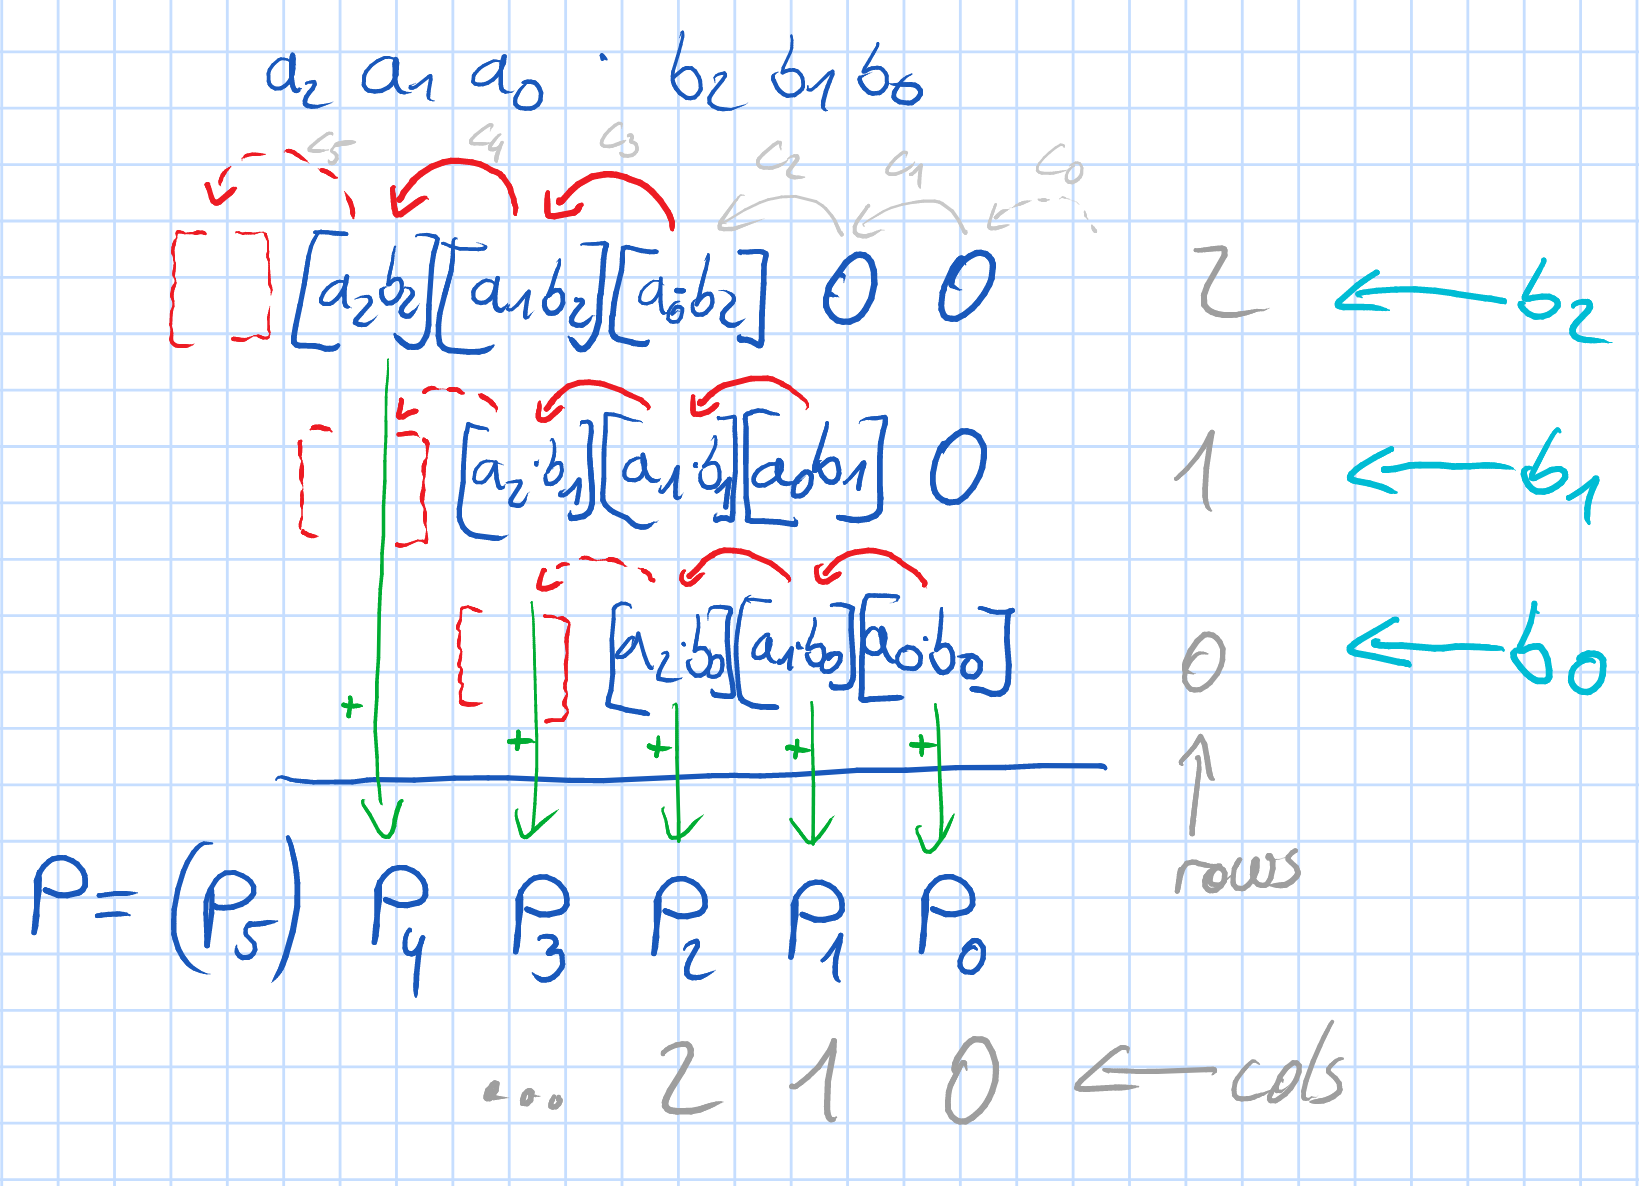
\includegraphics[width=0.7\linewidth]{images/opscanning}
        \caption{Veranschaulichung des Operand Scanning Ansatzes}
        \label{fig:opscanning}
    \end{figure}

\subsubsection{Product Scanning} \label{sec:prodscan}

    \paragraph*{Wichtige Funktionen}
    \begin{itemize} \tightlist
        \item Addition (s.o.)
        \item \ilc{MPint::prod\_scan\_mul(\&self, \dots) -> Self}
    \end{itemize}

    \paragraph*{Erklärung}
    Dieser Ansatz erspart das Vorhalten aller Teilprodukte und Überträge während der Berechnung. Stattdessen werden die einzelnen Produkt-Ziffern eine nach der anderen, \emph{direkt} berechnet.

    Das funktioniert deshalb, weil Ziffern der Operanden nur einen beschränkten Einflussbereich auf Ziffern des Produkts haben (vgl. \autoref{fig:prodscanningeinfluss}). Beispielsweise wird die erste Ziffer des Produkts ausschließlich von den beiden ersten Ziffern der Operanden beeinflusst. Bei der letzten Ziffer des Produkts verhält es sich analog, nur dass evtl. ein Übertrag aus den vorherigen Ziffern einfließt. Dementsprechend muss man von ,,rechts nach links'' durch das Produkt iterieren.

    Dabei betrachtet der implementierte Algorithmus die Operanden als hätten sie gleich viele Ziffern. Bei unterschiedlicher Anzahl wird der ,,kürzere'' Operand ggf. links mit Nullen aufgefüllt.

    Seien $a=a_{n}a_{n-1}\dots{}a_{1}a_{0}$ und $b=b_{n}b_{n-1}\dots{}b_{1}b_{0}$ die beiden Operanden.
    Da das Produkt $p = a \cdot b$ zweier Zahlen mit jeweils $n$ Ziffern höchstens $2 \cdot n$ Ziffern haben kann, gilt $p=p_{2n}p_{2 n-1}\dots{}p_{1}p_{0}$.

    Seien nun $i$ der Index, mit dem die einzelnen Ziffern des Produkts
    und $j$ der Index, mit dem die Ziffern beider Operanden referenziert werden.

    Aus besagtem Einflussbereich ergibt sich folgender Algorithmus zur Berechnung der einzelnen Produkt-Ziffern:
    \begin{enumerate}
        \item Sei $k=i-j$:
            \begin{itemize} \tightlist
                \item Falls $k \ge n$: Überspringe die aktuelle Operand-Ziffer ($j$)
                \item Falls $k < 0$: Ende des Einflussbereichs wurde erreicht. Gehe zur nächsten Produkt-Ziffer ($i$)
            \end{itemize}

        \item Die $i$-te Produkt-Ziffer $p_i$ wird berechnet als:
            \begin{itemize} \tightlist
                \item Summe aller Teilprodukte $p_{i,j} = a_j \cdot b_k$, wobei jedes offensichtlich bis zu 2 Ziffern ergeben kann (\ilc{u64 $\rightarrow$ u128})
                \item Addition des letzten Übertrags $c_{i-1}$
                \item Anschließende Modulo-Berechnung zur Basis des Zahlensystems.
            \end{itemize}
        \item Berechnen des Übertrags $c_{i}$ für die folgende Ziffer, als Quotient\footnote{Statt tatsächlich zu dividieren, wird hier einfach die ,,MSB-Hälfte'' der Bits des Zwischenergebnisses genommen.} aus  der obigen Gesamtsumme (vor Modulo-Berechnung).
    \end{enumerate}

    \begin{figure}[H]
        \centering
        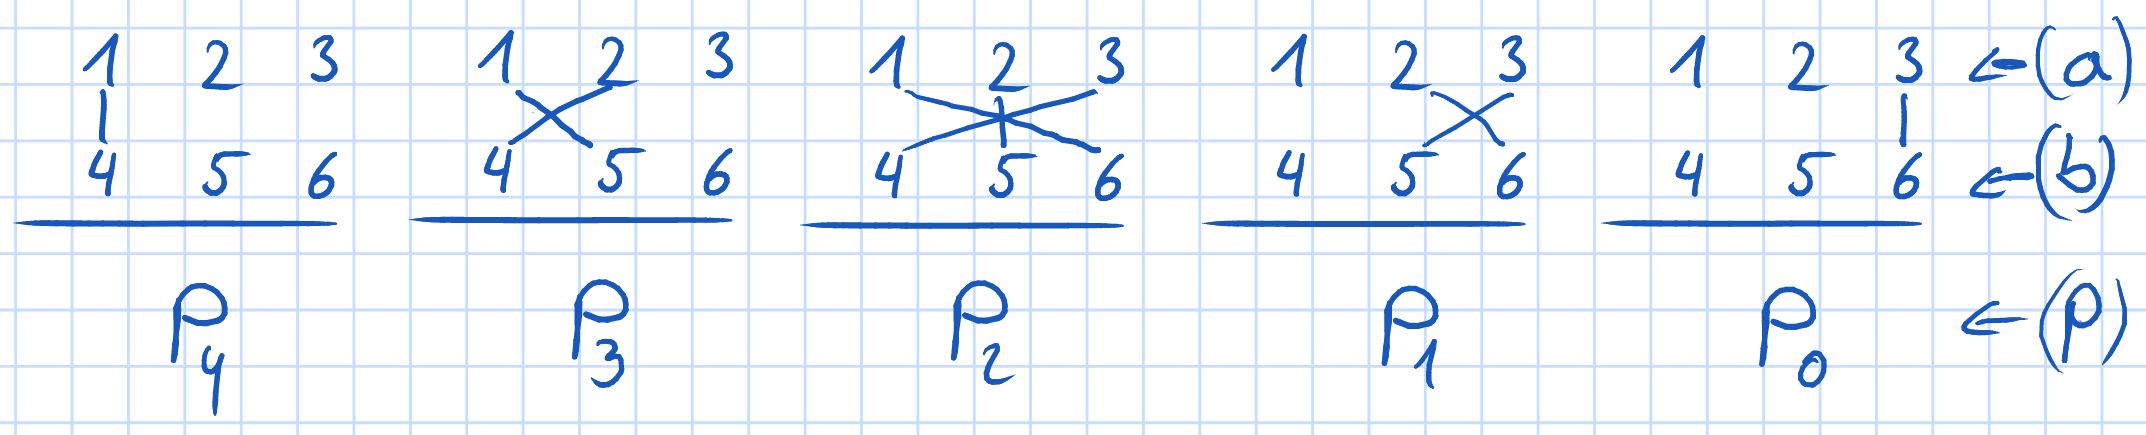
\includegraphics[width=0.7\linewidth]{images/prodscanningeinfluss}
        \caption{Veranschaulichung des Einflussbereichs der Ziffern beim Product Scanning Ansatz. $a$ und $b$ sind die Operanden, $p$ das Produkt. Die Linien zeigen, welche Ziffern in die jeweilige Produkt-Ziffer \emph{direkt} einfließen}
        \label{fig:prodscanningeinfluss}
    \end{figure}

